
\documentclass{beamer}

\newtheorem{conjecture}{Conjecture}
 \newcommand{\bconj}[1]{\begin{conj}#1\end{conj}}
\newtheorem{mconj}{Metaconjecture}

\newtheorem{prop}{Proposition}
 \newcommand{\bprop}[1]{\begin{prop}#1\end{prop}}
\newtheorem{lem}{Lemma}
 \newcommand{\blem}[1]{\begin{lem}#1\end{lem}}


\newtheorem{guess}{Guess}
 \newcommand{\bguess}[1]{\begin{guess}#1\end{guess}}
%\newtheorem{corollary}{Corollary}



\usepackage{tikz,framed, amsrefs, amsthm, color,wrapfig}
\tikzstyle{every node}=[circle, draw, fill=black!50,
                        inner sep=0pt, minimum width=4pt]
\tikzstyle{dot}=[circle, draw, fill=black,
                        inner sep=0pt, minimum width=2pt]

\tikzstyle{lblvertex}=[fill=white, inner sep = 1pt, font=\small]
\tikzstyle{lblvertex2}=[fill=white, inner sep = 1pt, font=\tiny,circle, draw]
\tikzstyle{lblvertex3}=[fill=white, inner sep = 1pt, font=\tiny,circle, draw = black!25]
\tikzstyle{words} =[rectangle, draw=none, fill=none, black]
\newcommand{\bframe}[2]{\begin{frame}{#1}#2\end{frame}}
\newcommand{\bfig}[2]{\begin{figure}#1\caption{#2}\end{figure}}


\usetheme{CambridgeUS}
\setbeamertemplate{navigation symbols}{}
\usecolortheme[RGB={216,30,5}]{structure}
\AtBeginSection[] % "Beamer, do the following at the start of every section"
{
\begin{frame}<beamer>
\frametitle{Outline} % make a frame titled "Outline"
\tableofcontents[currentsection] % show TOC and highlight current section
\end{frame}
}

\title{Connected matchings in special families of graphs}
\author{Chris Caragianis}
\institute[U of L]{ Department of Mathematics\\ University of Louisville\\ Louisville, KY 40292\\[1ex]
   \texttt{cjcara01@louisville.edu} }
\begin{document}

\bframe{}{\titlepage}

\bframe{}{\tableofcontents}

\section{Introduction}

\subsection{Review of graph-theoretic concepts}

\bframe{Graphs, vertex coloring}{
	\begin{overprint} 
		\onslide<1>A (simple, undirected) graph is a collection of \textit{vertices}, some pairs of which are \textit{adjacent}.  A pair of adjacent vertices is called an \textit{edge}. \\
		\onslide<2-3>A (simple, undirected) graph is a collection of \textit{vertices}, some pairs of which are \textit{adjacent}.  A pair of adjacent vertices is called an \textit{edge}. \vskip 0.5 cm A proper vertex coloring is one in which adjacent vertices recieve different colors.
	\end{overprint}	
	\vskip 1 cm 
		\only<1-2>{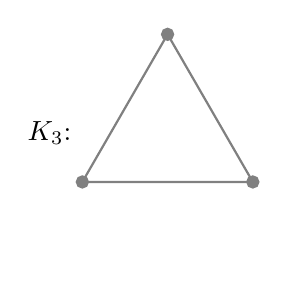
\begin{tikzpicture}[thick,scale=0.5]
\draw[gray] 
    {
		(180:3) node[words] {$K_3$:}
        (90:2.5) node {}  -- (210:2.5)
		(210:2.5) node {} -- (-30:2.5)
		(-30:2.5) node {} -- (90:2.5)
		(-90:3.5) node[words] {}
    };

\end{tikzpicture}
}\only<3>{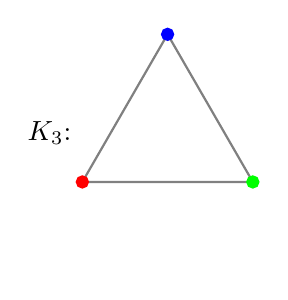
\begin{tikzpicture}[thick,scale=0.5]
\draw[gray] 
    {
		(180:3) node[words] {$K_3$:}
        (90:2.5) node[blue] {}  -- (210:2.5)
		(210:2.5) node[red] {} -- (-30:2.5)
		(-30:2.5) node[green] {} -- (90:2.5)
		(-90:3.5) node[words] {}
    };

\end{tikzpicture}
} \qquad 
		\only<1-2>{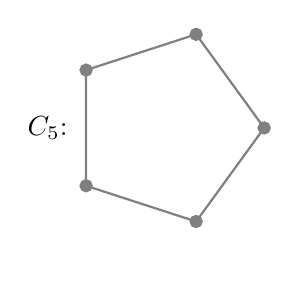
\begin{tikzpicture}[thick,scale=0.5]
\draw[gray] 
    {
		(180:3) node[words] {$C_5$:}
        (72:2.5) node {}  -- (144:2.5)
		(144:2.5) node {} -- (216:2.5)
		(216:2.5) node {} -- (288:2.5)
		(288:2.5) node {}  -- (0:2.5)
		(0:2.5) node {} -- (72:2.5)
		(-90:3.5) node[words] {}
    };
	
\end{tikzpicture}
}\only<3>{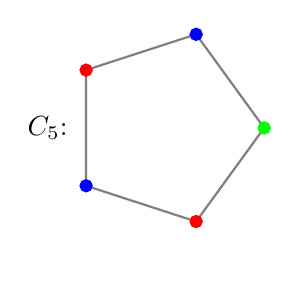
\begin{tikzpicture}[thick,scale=0.5]
\draw[gray] 
    {
		(180:3) node[words] {$C_5$:}
        (72:2.5) node[blue] {}  -- (144:2.5)
		(144:2.5) node[red] {} -- (216:2.5)
		(216:2.5) node[blue] {} -- (288:2.5)
		(288:2.5) node[red] {}  -- (0:2.5)
		(0:2.5) node[green] {} -- (72:2.5)
		(-90:3.5) node[words] {}
    };
	
\end{tikzpicture}
} \qquad 
		\only<1-2>{\begin{tikzpicture}[thick,scale=0.5]
\draw[gray] 
    {
		(180:3) node[words] {$G$:}
        (90:2.5) node {}  -- (0:0)
		(210:2.5) node {} -- (0:0)
		(-30:2.5) node {} -- (0:0)
		(0:0) node {}
		(-90:3.5) node[words] {}
    };

\end{tikzpicture}
}\only<3>{\begin{tikzpicture}[thick,scale=0.5]
\draw[gray] 
    {
		(180:3) node[words] {$G$:}
        (90:2.5) node[red] {}  -- (0:0)
		(210:2.5) node[red] {} -- (0:0)
		(-30:2.5) node[red] {} -- (0:0)
		(0:0) node[blue] {}
		(-90:3.5) node[words] {}
    };

\end{tikzpicture}
}
}

\bframe{Clique number, independence number}{
	\begin{itemize}
		\item A \textit{clique} on $n$ vertices (also called a \textit{complete graph}) is a collection of $n$ vertices along with all possible edges.\pause  
		\item The \textit{clique number} of $G$, denoted $\omega(G)$, is the size of the largest clique in $G$.\pause  
		\item The \textit{independence number} of $G$, denoted $\alpha(G)$, is the size of the largest set of vertices from $G$ that induces no edges.\pause
	\end{itemize}
	\begin{center}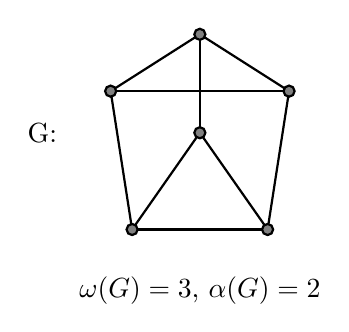
\begin{tikzpicture}[thick,scale=0.5]

	\coordinate (a) at (90:2.5);
	\coordinate (b) at (25:2.5); 
	\coordinate (c) at (0:0);
	\coordinate (d) at (155:2.5);
	\coordinate (e) at (-55:3);
	\coordinate (f) at (-125:3);

	\draw (a)--(b);
	%\draw (b)--(c);
	\draw (d)--(a);
	\draw (a)--(c);
	%\draw (c)--(d);
	\draw (b)--(e);
	\draw (e)--(c);
	\draw (d)--(f);
	\draw (f)--(c);
	\draw (d)--(b);
	\draw (e)--(f);
	%\draw (f) arc {-125:-33:3};
	
	\draw (a) node {};
	\draw (b) node {};
	\draw (c) node {};
	\draw (d) node {};
	\draw (e) node {};
	\draw (f) node {};
	\draw (-90:4) node[words] {$\omega(G) = 3$, $\alpha(G) = 2$};
	\draw (180:4) node[words] {G:};
\end{tikzpicture}
\end{center}}

\bframe{Chromatic number}{The \textit{chromatic number} of a graph $G$, denoted $\chi(G)$, is the minimum number of colors needed to properly color the vertices of $G$.
	\begin{overprint}	
		\onslide<1>\vskip 1 cm 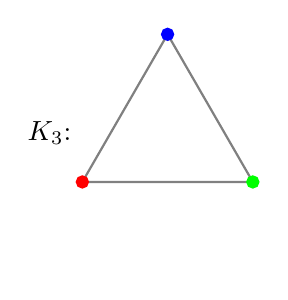
\begin{tikzpicture}[thick,scale=0.5]
\draw[gray] 
    {
		(180:3) node[words] {$K_3$:}
        (90:2.5) node[blue] {}  -- (210:2.5)
		(210:2.5) node[red] {} -- (-30:2.5)
		(-30:2.5) node[green] {} -- (90:2.5)
		(-90:3.5) node[words] {}
    };

\end{tikzpicture}
 \qquad 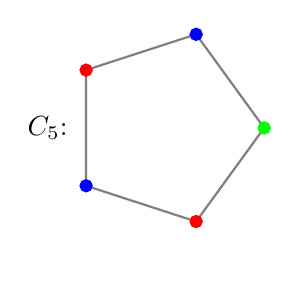
\begin{tikzpicture}[thick,scale=0.5]
\draw[gray] 
    {
		(180:3) node[words] {$C_5$:}
        (72:2.5) node[blue] {}  -- (144:2.5)
		(144:2.5) node[red] {} -- (216:2.5)
		(216:2.5) node[blue] {} -- (288:2.5)
		(288:2.5) node[red] {}  -- (0:2.5)
		(0:2.5) node[green] {} -- (72:2.5)
		(-90:3.5) node[words] {}
    };
	
\end{tikzpicture}
 \qquad \begin{tikzpicture}[thick,scale=0.5]
\draw[gray] 
    {
		(180:3) node[words] {$G$:}
        (90:2.5) node[red] {}  -- (0:0)
		(210:2.5) node[red] {} -- (0:0)
		(-30:2.5) node[red] {} -- (0:0)
		(0:0) node[blue] {}
		(-90:3.5) node[words] {}
    };

\end{tikzpicture}
\\
		\onslide<2>\vskip 1 cm 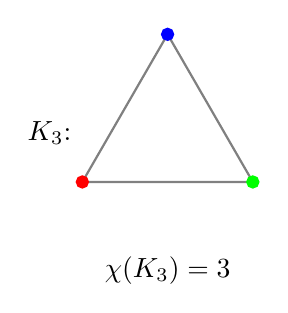
\begin{tikzpicture}[thick,scale=0.5]
\draw[gray] 
    {	
		(180:3) node[words] {$K_3$:}
        (90:2.5) node[blue] {}  -- (210:2.5)
		(210:2.5) node[red] {} -- (-30:2.5)
		(-30:2.5) node[green] {} -- (90:2.5)
		(-90:3.5) node[words] {$\chi(K_3) = 3$}
    };

\end{tikzpicture}
 \qquad 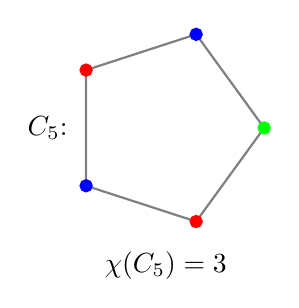
\begin{tikzpicture}[thick,scale=0.5]
\draw[gray] 
    {
		(180:3) node[words] {$C_5$:}
        (72:2.5) node[blue] {}  -- (144:2.5)
		(144:2.5) node[red] {} -- (216:2.5)
		(216:2.5) node[blue] {} -- (288:2.5)
		(288:2.5) node[red] {}  -- (0:2.5)
		(0:2.5) node[green] {} -- (72:2.5)
		(-90:3.5) node[words] {$\chi(C_5) = 3$}
    };
	
\end{tikzpicture}
 \qquad 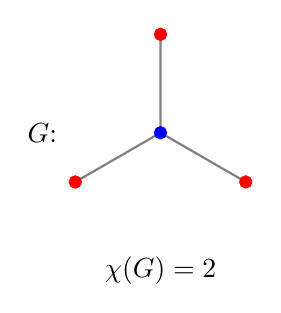
\begin{tikzpicture}[thick,scale=0.5]
\draw[gray] 
    {
		(180:3) node[words] {$G$:}
        (90:2.5) node[red] {}  -- (0:0)
		(210:2.5) node[red] {} -- (0:0)
		(-30:2.5) node[red] {} -- (0:0)
		(0:0) node[blue] {}
		(-90:3.5) node[words] {$\chi(G) = 2$}
    };

\end{tikzpicture}

	\end{overprint}}

\subsection{Connected matchings}

\bframe{Connected matchings}{
 A {\it matching} in a graph $G$ is a collection of disjoint edges. \pause\vskip 0.5 cm
 A \textit{connected matching} is a collection of disjoint edges such that each pair of edges has a pair of adjacent endpoints. \pause
	\begin{center}
	\begin{overprint}
		\onslide<2>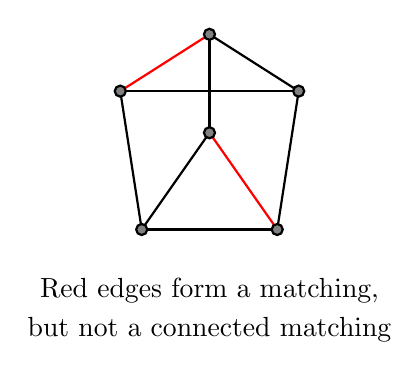
\begin{tikzpicture}[thick,scale=0.5]

	\coordinate (a) at (90:2.5);
	\coordinate (b) at (25:2.5); 
	\coordinate (c) at (0:0);
	\coordinate (d) at (155:2.5);
	\coordinate (e) at (-55:3);
	\coordinate (f) at (-125:3);

	\draw (a)--(b);
	%\draw (b)--(c);
	\draw[red] (d)--(a);
	\draw (a)--(c);
	%\draw (c)--(d);
	\draw (b)--(e);
	\draw[red] (e)--(c);
	\draw (d)--(f);
	\draw (f)--(c);
	\draw (d)--(b);
	\draw (e)--(f);
	%\draw (f) arc {-125:-33:3};
	
	\draw (a) node {};
	\draw (b) node {};
	\draw (c) node {};
	\draw (d) node {};
	\draw (e) node {};
	\draw (f) node {};
	\draw (-90:4) node[words] {Red edges form a matching,};
	\draw (-90:5) node[words] {but not a connected matching};
\end{tikzpicture}
\\
		\onslide<3-> 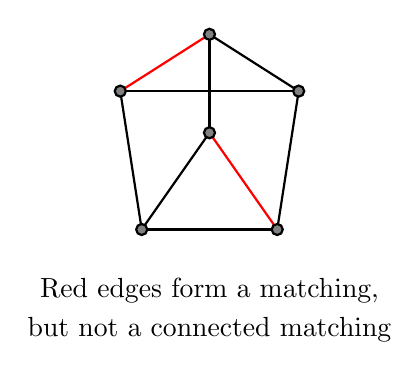
\begin{tikzpicture}[thick,scale=0.5]

	\coordinate (a) at (90:2.5);
	\coordinate (b) at (25:2.5); 
	\coordinate (c) at (0:0);
	\coordinate (d) at (155:2.5);
	\coordinate (e) at (-55:3);
	\coordinate (f) at (-125:3);

	\draw (a)--(b);
	%\draw (b)--(c);
	\draw[red] (d)--(a);
	\draw (a)--(c);
	%\draw (c)--(d);
	\draw (b)--(e);
	\draw[red] (e)--(c);
	\draw (d)--(f);
	\draw (f)--(c);
	\draw (d)--(b);
	\draw (e)--(f);
	%\draw (f) arc {-125:-33:3};
	
	\draw (a) node {};
	\draw (b) node {};
	\draw (c) node {};
	\draw (d) node {};
	\draw (e) node {};
	\draw (f) node {};
	\draw (-90:4) node[words] {Red edges form a matching,};
	\draw (-90:5) node[words] {but not a connected matching};
\end{tikzpicture}
\qquad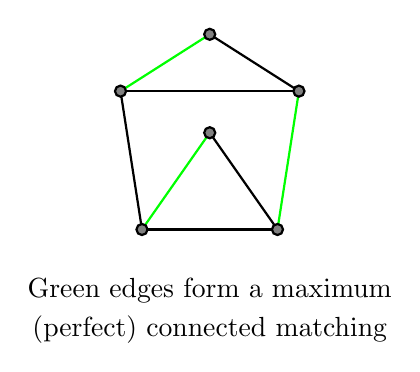
\begin{tikzpicture}[thick,scale=0.5]

	\coordinate (a) at (90:2.5);
	\coordinate (b) at (25:2.5); 
	\coordinate (c) at (0:0);
	\coordinate (d) at (155:2.5);
	\coordinate (e) at (-55:3);
	\coordinate (f) at (-125:3);

	\draw (a)--(b);
	%\draw (b)--(c);
	\draw[green] (d)--(a);
	%\draw (a)--(c);
	%\draw (c)--(d);
	\draw[green] (b)--(e);
	\draw (e)--(c);
	\draw (d)--(f);
	\draw[green] (f)--(c);
	\draw (d)--(b);
	\draw (e)--(f);
	%\draw (f) arc {-125:-33:3};
	
	\draw (a) node {};
	\draw (b) node {};
	\draw (c) node {};
	\draw (d) node {};
	\draw (e) node {};
	\draw (f) node {};
	\draw (-90:4) node[words] {Green edges form a maximum};
	\draw (-90:5) node[words] {(perfect) connected matching};
\end{tikzpicture}

	\end{overprint}
	\end{center}\pause
We will denote by $\nu_c(G)$ the size of a maximum connected matching in $G$.
}

\bframe{Problems}{
The problems we will be looking at fall into two categories\pause\vskip 0.5 cm 
\begin{itemize}
	\item Extremal: How many vertices must a graph $G$ (under proper conditions) have in order to guarantee the presence of a conneceted matching of a given size?\pause\vskip 0.5 cm 
	\item Computational: How may we find the size of a maximum connected matching in $G$?
\end{itemize}
}

\bframe{Separable edges, Neighborly edges}{

If a pair of edges $e $ and $f$ from a graph $G$ are disjoint and have no pair of adjacent endpoints then we say that $e$ and $f$ are {\it separable}. \pause\vskip 0.5 cm

Otherwise, we say $e$ and $f$ are {\it neighborly}. \pause\vskip 0.5 cm
\begin{center}
	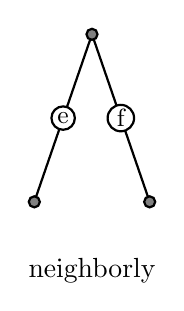
\begin{tikzpicture}[thick,scale=0.75]

	\coordinate (a0) at (0:0);
	\coordinate (a1) at (180:1);
	\coordinate (a3) at (-109:3);
	\coordinate (a2) at (0:1);
	\coordinate (a4) at (-71:3);
	\coordinate (text) at (-90:4);
	\coordinate (b2) at (30:3);

	\draw (a0)-- node[lblvertex] {e}(a3);
	\draw (a0)-- node[lblvertex] {f}(a4);

	\draw (a0) node {};	
	\draw (text) node[words] {neighborly};
	\draw (a3) node {};
	\draw (a4) node {};
	
\end{tikzpicture}
\qquad\pause
	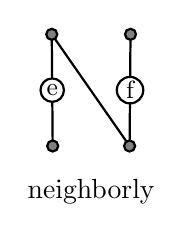
\begin{tikzpicture}[thick,scale=0.5]

	\coordinate (a0) at (0:0);
	\coordinate (a1) at (180:1);
	\coordinate (a3) at (-109:3);
	\coordinate (a2) at (0:1);
	\coordinate (a4) at (-71:3);
	\coordinate (text) at (-90:4);
	\coordinate (b2) at (30:3);

	\draw (a1)-- node[lblvertex] {e}(a3);
	\draw (a2)-- node[lblvertex] {f}(a4);
	\draw (a1)--(a4);
	\draw (a1) node[]{};
	\draw (a2) node[]{};
	\draw (a3) node[]{};
	\draw (a4) node[]{};
	\draw (text) node[words] {neighborly};
\end{tikzpicture}
\qquad\pause
	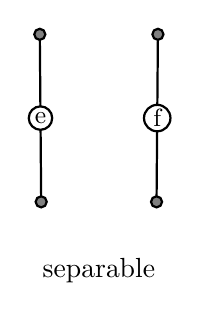
\begin{tikzpicture}[thick,scale=0.75]

	\coordinate (a0) at (0:0);
	\coordinate (a1) at (180:1);
	\coordinate (a3) at (-109:3);
	\coordinate (a2) at (0:1);
	\coordinate (a4) at (-71:3);
	\coordinate (b1) at (150:3);
	\coordinate (text) at (-90:4);

	\draw (a1)-- node[lblvertex] {e}(a3);
	\draw (a2)-- node[lblvertex] {f}(a4);
	\draw (a1) node[]{};
	\draw (a2) node[]{};
	\draw (a3) node[]{};
	\draw (a4) node[]{};
	\draw (text) node[words] {separable};
	
\end{tikzpicture}
 \pause
\end{center}
\vskip 0.5 cm
A graph that contains a separable pair of edges is called separable.  \pause A connected matching is a matching which contains no separable pair.

}


\section{Connected matchings and Hadwiger's conjecture}

\subsection{Hadwiger's conjecture}

\bframe{Perfect graphs}{
	For any graph $G$, $\chi(G) \geq \omega(G)$\pause, but the converse is not true.\pause
\begin{center}
 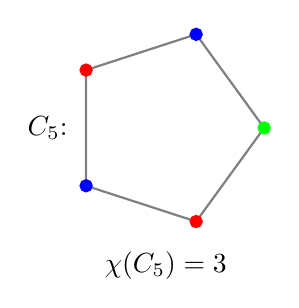
\begin{tikzpicture}[thick,scale=0.5]
\draw[gray] 
    {
		(180:3) node[words] {$C_5$:}
        (72:2.5) node[blue] {}  -- (144:2.5)
		(144:2.5) node[red] {} -- (216:2.5)
		(216:2.5) node[blue] {} -- (288:2.5)
		(288:2.5) node[red] {}  -- (0:2.5)
		(0:2.5) node[green] {} -- (72:2.5)
		(-90:3.5) node[words] {$\chi(C_5) = 3$}
    };
	
\end{tikzpicture}
 
\end{center}
\pause

	We say that a graph $G$ is \textit{perfect} if for every induced subgraph $H$ of $G$, $\chi(H) = \omega(H)$.\pause 
\begin{theorem}[Strong perfect graph theorem (SPGT)]A graph $G$ is perfect if and only if for each $k >1$ it has neither a $C_{2k+1}$ nor its complement as an induced subgraph.\end{theorem}}

\bframe{Toft's ``metaconjecture''}{

Is there a structure in graphs the size of which provides an {\it upper } bound to the chromatic number?\pause\vskip 0.5 cm 

Bjarne Toft framed the question in this way \cite{MR1411244}: \pause
\begin{mconj}
The largest number of colors needed to color any graph in a topological class is precisely the largest number of vertices in any complete graph belonging to the class
\end{mconj}\pause\vskip 0.25 cm 
One way of defining ``topological class'' is using {\it graph minors}.
}


\bframe{Graph minors}{We say that a graph $G$ contains $H$ \textit{as a minor}, (denoted $G\geq H$), if $H$ is obtained from $G$ by successive vertex deletions and edge contractions.\pause \vskip 0.5 cm
An ``edge contraction'' consists of identifying two adjacent vertices, the resulting vertex being adjacent to any neighbors of either.\pause

\begin{center}
 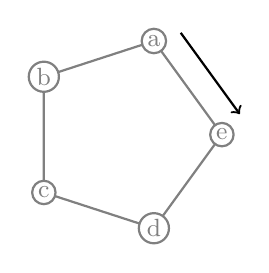
\begin{tikzpicture}[thick,scale=0.5]
\draw[gray] 
    {
        (72:2.5) node[lblvertex] {a}  -- (144:2.5)
		(144:2.5) node[lblvertex] {b} -- (216:2.5)
		(216:2.5) node[lblvertex] {c} -- (288:2.5)
		(288:2.5) node[lblvertex] {d}  -- (0:2.5)
		(0:2.5) node[lblvertex] {e} -- (72:2.5)
		
	
    };
	\draw (62:3)node[words] {}
		edge[->] (10:3);
	
\end{tikzpicture}
 \quad\pause
 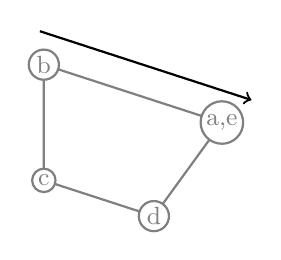
\begin{tikzpicture}[thick,scale=0.5]
\draw[gray] 
    {
        
		(144:2.5) node[lblvertex] {b} -- (216:2.5)
		(216:2.5) node[lblvertex] {c} -- (288:2.5)
		(288:2.5) node[lblvertex] {d}  -- (0:2.5)
		(0:2.5) node[lblvertex] {a,e} -- (144:2.5)
	
    };
	\draw (134:3.3)node[words] {}
		edge[->] (10:3.3);
	
\end{tikzpicture}
\quad\pause
 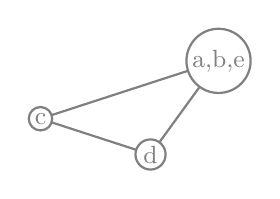
\begin{tikzpicture}[thick,scale=0.5]
\draw[gray] 
    {
        
		
		(216:2.5) node[lblvertex] {c} -- (288:2.5)
		(288:2.5) node[lblvertex] {d}  -- (0:2.5)
		(0:2.5) node[lblvertex] {a,b,e} -- (216:2.5)
	
    };
	
	
\end{tikzpicture}
\pause
\vskip 0.25 cm 
$C_5 \geq K_3$
\end{center}

	 }

\bframe{Hadwiger's conjecture}{
    It is widely believed, but is yet to be proved, that the size of the largest complete minor in a graph is an upper bound on the chromatic number. \pause
\vskip 0.5 cm Formally, let $\eta(G)$ be the largest $n$ for which $G \geq K_n$.\pause
 \vskip 0.5 cm \begin{conjecture}[Hadwiger, 1943] For all graphs $G$, \[\eta(G) \geq \chi(G)\] 
\end{conjecture}
 }

\subsection{A weaker conjecture than Hadwigers}

\bframe{A weaker conjecture.}{

	For all graphs $G$ on $n$ vertices, $n/\alpha(G) \leq \chi(G)$.\pause\vskip 0.5 cm
 The following conjecture is then implied by Hadwiger's.\pause
\begin{conjecture}\label{hc}
 For any graph $G$ on $n$ vertices with $\alpha(G) =\alpha$, \[\eta(G) \geq \frac{n}{\alpha}\]
\end{conjecture}
\pause \vskip 0.25 cm

Plummer, Stiebitz and Toft  show in \cite{MR2070161} that this is equivalent to Hadwiger's conjecture for graphs with independence number two.

}

\bframe{}{
\begin{conjecture}\label{hc}
 For any graph $G$ on $n$ vertices with $\alpha(G) =\alpha$, \[\eta(G) \geq \frac{n}{\alpha}\]
\end{conjecture}\pause
 Duchet and Meyniel showed in  \cite{MR671905} (1982) that $\displaystyle\eta(G) \geq \frac{ n}{2\alpha - 1}$.\pause \vskip 0.5 cm 

When $\alpha \geq 3$, Kawarabayashi, Plummer and Toft \cite{MR2156345} improve this to 
\[\eta(G) \geq \frac{n(4\alpha-2)}{(4\alpha-3)(2\alpha -1)}\].   \pause  When $\alpha = 2$, the result of Duchet and Meyniel is still the best known. \pause \vskip 0.5 cm

The problem of reducing the constant of $1/3$ in the $\alpha  = 2 $ case remains. 
}

\subsection{Connected matchings in $\alpha = 2$ graphs}

\bframe{An extremal conjecture for connected matchings}{
  Gy\'arf\'as, F\"uredi and Simonyi observe this and conjecture \pause 
 	\begin{conjecture}[2005]
  		There exists an absolute constant $c$ so that any graph $G$ with $\alpha(G) =2$ and at least $ct$ vertices has a connected matching of at least $t$ edges.
 	\end{conjecture}\vskip 0.5 cm\pause
 	If true, this would imply that when $\alpha(G) = 2$, $\eta(G) > n/3$. \pause\vskip 0.5 cm 
 They further conjecture that $c = 4$ and prove this for $t \leq 17$.}

\bframe{Partial results}{

We have the following partial results toward resolving this conjecture.
\pause \vskip 0.5 cm
Fix $c < 1/4$ and let $G$ be a graph on $n$ vertices with $\alpha(G) = 2$ and no connected matching of size $cn$. \pause \vskip 0.25 cm
\begin{enumerate}
	\item $\omega(G) < cn$ \pause (Plummer et. al. CITE) \pause
	\item $G$ is $\displaystyle\left( \frac{c-1}{c}\right)n$ connected \pause (Extends a result of Blasiak \cite{blas})\pause
	\item For any constant $b$ and $n$ sufficiently large, $\omega(G) \geq b\sqrt{n\log n}$  
\end{enumerate}
}

\bframe{}{
We will delay the proof of 3 until introducing some useful notation.
}

\section{Proximity Partitions}

\subsection{Basic facts and definitions}

\bframe{Line graphs}{
	Recall the definition of a line graph.\pause\vskip 0.5 cm

	For any graph $G$, the \textit{line graph} of $G$, denoted $L(G)$, is the graph with vertex set equal to the edge set of $G$, with edges between vertices corresponding to incident edges in $G$.\pause\vskip 0.5 cm

	\begin{center}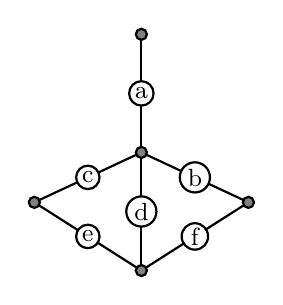
\begin{tikzpicture}[thick,scale=0.5]

	\coordinate (a1) at (90:3);
	\coordinate (a2) at (-25:3); 
	\coordinate (a3) at (-155:3);
	\coordinate (a4) at (-90:3);
	\coordinate (a5) at (0:0);

	\draw (a5)-- node [lblvertex] {a}(a1);
	\draw (a5)-- node [lblvertex] {b}(a2);
	\draw (a5)-- node [lblvertex] {c}(a3);
	\draw (a5)-- node [lblvertex] {d}(a4);
	\draw (a3)-- node [lblvertex] {e}(a4);
	\draw (a2)-- node [lblvertex] {f}(a4);

	\draw (a1) node {};
	\draw (a2) node {};
	\draw (a3) node {};
	\draw (a4) node {};
	\draw (a5) node {};
	%\draw (a1) node[lblvertex] {a};
	%\draw (a2) node[lblvertex] {b};  
	
\end{tikzpicture}
\pause\quad 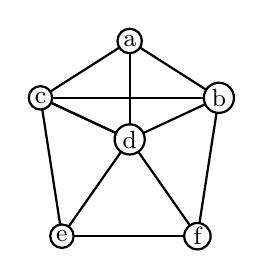
\begin{tikzpicture}[thick,scale=0.5]

	\coordinate (a) at (90:2.5);
	\coordinate (b) at (25:2.5); 
	\coordinate (c) at (0:0);
	\coordinate (d) at (155:2.5);
	\coordinate (e) at (-55:3);
	\coordinate (f) at (-125:3);

	\draw (a)--(b);
	\draw (b)--(c);
	\draw (c)--(d);
	\draw (d)--(a);
	\draw (a)--(c);
	\draw (c)--(d);
	\draw (b)--(e);
	\draw (e)--(c);
	\draw (d)--(f);
	\draw (f)--(c);
	\draw (d)--(b);
	\draw (e)--(f);
	%\draw (f) arc {-125:-33:3};
	
	\draw (a) node [lblvertex]{a};
	\draw (b) node [lblvertex]{b};
	\draw (c) node [lblvertex]{d};
	\draw (d) node [lblvertex]{c};
	\draw (e) node [lblvertex]{f};
	\draw (f) node [lblvertex]{e};
\end{tikzpicture}
\end{center}}
\bframe{Connected matching as a clique problem}{
	Let $G$ be a graph with $m$ edges.  \pause We can color the edges of $K_m$ in this way:\pause
	\begin{itemize} 
		\uncover<3->{\item Blue edges correspond to a pair of incident edges in $G$ (i.e., $L(G)$)} 
	 	\uncover<5->{\item Green edges correspond to a pair of disjoint edges in $G$ with some edge between them,} 
		\uncover<7->{\item Red edges correspond to separable edges.}
	\end{itemize}
	\begin{center}
		\uncover<4->{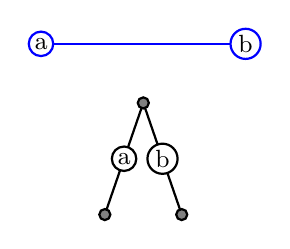
\begin{tikzpicture}[thick,scale=0.5]

	\coordinate (a0) at (0:0);
	\coordinate (a1) at (180:1);
	\coordinate (a3) at (-109:3);
	\coordinate (a2) at (0:1);
	\coordinate (a4) at (-71:3);
	\coordinate (b1) at (150:3);
	\coordinate (b2) at (30:3);

	\draw (a0)-- node[lblvertex] {a}(a3);
	\draw (a0)-- node[lblvertex] {b}(a4);
	\draw (b1)[blue]--(b2);
	\draw (a0) node {};	
	%\draw (a1) node {};
	%\draw (a2) node {};
	\draw (a3) node {};
	\draw (a4) node {};
	\draw (b1) node[lblvertex, draw = blue] {a};
	\draw (b2) node[lblvertex, draw = blue] {b};
\end{tikzpicture}
}\uncover<6->{\qquad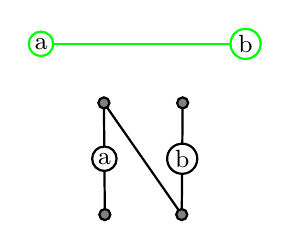
\begin{tikzpicture}[thick,scale=0.5]

	\coordinate (a0) at (0:0);
	\coordinate (a1) at (180:1);
	\coordinate (a3) at (-109:3);
	\coordinate (a2) at (0:1);
	\coordinate (a4) at (-71:3);
	\coordinate (b1) at (150:3);
	\coordinate (b2) at (30:3);

	\draw (a1)-- node[lblvertex] {a}(a3);
	\draw (a2)-- node[lblvertex] {b}(a4);
	\draw (a1)--(a4);
	\draw (b1)[green]--(b2);
	%\draw (a0) node {};	
	\draw (a1) node {};
	\draw (a2) node {};
	\draw (a3) node {};
	\draw (a4) node {};
	\draw (b1) node [lblvertex, draw = green]{a};
	\draw (b2) node [lblvertex, draw = green]{b};
\end{tikzpicture}
}\uncover<8->{\qquad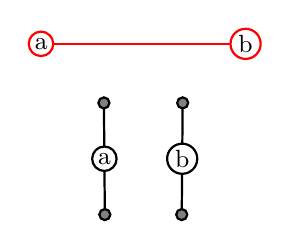
\begin{tikzpicture}[thick,scale=0.5]

	\coordinate (a0) at (0:0);
	\coordinate (a1) at (180:1);
	\coordinate (a3) at (-109:3);
	\coordinate (a2) at (0:1);
	\coordinate (a4) at (-71:3);
	\coordinate (b1) at (150:3);
	\coordinate (b2) at (30:3);

	\draw (a1)-- node[lblvertex] {a}(a3);
	\draw (a2)-- node[lblvertex] {b}(a4);
	%\draw (a1)--(a4);
	\draw (b1)[red]--(b2);
	%\draw (a0) node {};	
	\draw (a1) node {};
	\draw (a2) node {};
	\draw (a3) node {};
	\draw (a4) node {};
	\draw (b1) node[lblvertex, draw = red] {a};
	\draw (b2) node[lblvertex, draw = red] {b};
\end{tikzpicture}
}
	\end{center}\vskip 0.25 cm 
\uncover<9>{Connected matchings in $G$ then correspond to cliques in the green graph induced by $G$.}}

\bframe{}{

We now restate our third partial result. \pause\vskip 0.5 cm
\begin{theorem}
Let $c < 1/4$ be a constant.  For any constant $b$ and sufficently large $n$, every graph $G$ on $n$ vertices with $m$ edges, $\alpha(G) = 2$, and $\omega(G) < b\sqrt{n\log n}$ has a $cn$-connected matching.
\label{sm_cli}
\end{theorem}
\pause\vskip 0.5 cm
We will refer to the coloring of $K_m$ just described.  \pause\vskip 0.8 cm
We will show that (for large $n$) unless the clique number of $G$ is sufficiently large, the green graph induced by $G$ has too many edges to avoid a $cn$ clique. 
}

\bframe{}{

First, a lemma about triangle free graphs.\pause\vskip 0.5 cm 
\blem{For every pair of positive constants $\epsilon, d$ there is $n_{\epsilon, d}$ such that every triangle-free graph $G$ with $n > n_{\epsilon, d}$ vertices and $\alpha(G) < d\sqrt{n\log n}$ has fewer than $\epsilon n^3$ induced copies of $C_4$.}\pause \vskip 0.5 cm

Fix $\epsilon, d> 0$ and let $G$ be a triangle free graph on $n$ vertices with $\alpha(G) < d\sqrt{n\log n}$. \pause \vskip 0.8 cm
Let $X_{C_4}$ be the number of induced $C_4$s in $G$.  

}

\bframe{Proof of Lemma: Counting induced $C_4$s}{
\pause
\begin{center}
\begin{overprint}
	\onslide<2>\hspace{3.5cm}\begin{tikzpicture}[thick,scale=0.4]

\draw (-4,4) node[lblvertex]{x}
		edge[dashed] (4,4);
\draw(4,4) node[lblvertex]{y}; 
	
\draw[color = white](-2,-2) ellipse(4 and 2);
\draw[color = white](2,-2) ellipse(4 and 2);
	
\end{tikzpicture}
\\
	\onslide<3>\hspace{3.5cm}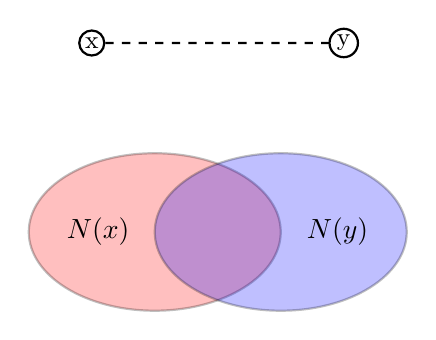
\begin{tikzpicture}[thick,scale=0.4]

\draw (-4,4) node[lblvertex]{x}
 	edge[dashed] (4,4);	
\draw(4,4) node[lblvertex]{y}; 
	
\draw[fill = red, opacity = 0.25](-2,-2) ellipse (4 cm  and 2.5 cm);
\draw[fill = blue, opacity = 0.25](2,-2) ellipse (4 cm and 2.5 cm);

\draw (-3.8,-2) node[words]{$N(x)$};
\draw (3.8,-2) node[words]{$N(y)$};
\end{tikzpicture}
\\
	\onslide<4>\hspace{3.5cm}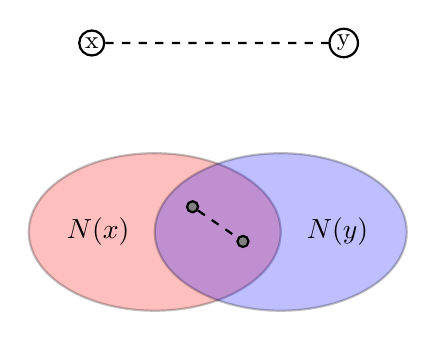
\begin{tikzpicture}[thick,scale=0.4]

\draw (-4,4) node[lblvertex]{x}
	edge[dashed] (4,4);
\draw(4,4) node[lblvertex]{y}; 
	
\draw[fill = red, opacity = 0.25](-2,-2) ellipse (4 cm  and 2.5 cm);
\draw[fill = blue, opacity = 0.25](2,-2) ellipse (4 cm and 2.5 cm);

\draw (-3.8,-2) node[words]{$N(x)$};
\draw (3.8,-2) node[words]{$N(y)$};

\draw (-.8,-1.2) node[]{}
	edge[dashed] (.8,-2.3);
\draw (.8,-2.3) node[]{};

\end{tikzpicture}\\
	\onslide<5->\hspace{3.5cm}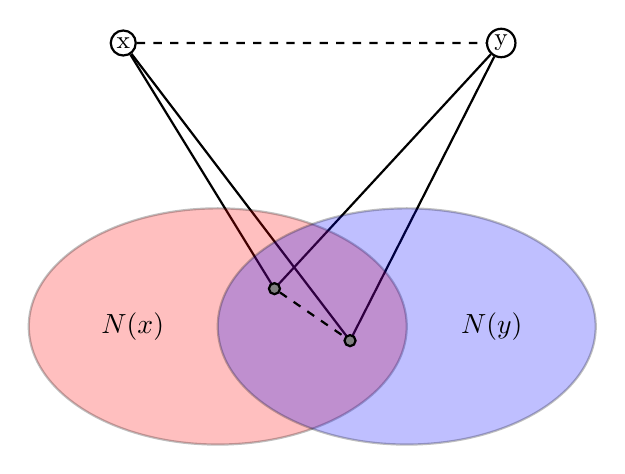
\begin{tikzpicture}[thick,scale=0.6]

\draw (-4,4) node[lblvertex]{x}
	edge[dashed] (4,4)
	edge[] (-.8,-1.2)
	edge[] (.8, -2.3);
	
\draw(4,4) node[lblvertex]{y}
	edge[] (-.8,-1.2)
	edge[] (.8, -2.3); 
	
\draw[fill = red, opacity = 0.25](-2,-2) ellipse (4 cm  and 2.5 cm);
\draw[fill = blue, opacity = 0.25](2,-2) ellipse (4 cm and 2.5 cm);

\draw (-3.8,-2) node[words]{$N(x)$};
\draw (3.8,-2) node[words]{$N(y)$};

\draw (-.8,-1.2) node[]{}
	edge[dashed] (.8,-2.3);
\draw (.8,-2.3) node[]{};

\end{tikzpicture}
\end{overprint}
\end{center}
\uncover<6->{\[X_{C_4} = \frac{1}{2}\sum_{\{u,v\}\notin E(G)} {|N(u) \cap N(v)| \choose 2}\]}
\uncover<7>{Set $\epsilon_1 < \sqrt{8\epsilon}$.}
}


	\bframe{Proof of Lemma, Bounding \# of large nbd intersections}{\pause
\vspace{-4pt}
\begin{framed} Claim. \textit{For sufficiently large $n$, fewer than $n^2(\log n)^{-2}$ pairs of vertices $u,v$ have neighborhood intersection larger than $\epsilon_1\sqrt{n}$.}
\end{framed}\pause \vskip 1 cm
Suppose the contrary is true, and there are more than $n^2(\log n)^{-2}$ pairs $u,v$ so that $|N(u)\cap N(v)| \geq \epsilon_1\sqrt{n}$. \pause \vskip 0.5 cm
Total vertex count\hspace{10pt}\pause $\geq\:\epsilon_1n^{5/2}(\log n)^{-2}$\pause \vskip 0.5 cm
Some vertex must have been counted at least $\epsilon_1n^{3/2}(\log n)^{-2}$ times. 
}

\bframe{Proof of Lemma, Bounding \# of large nbd intersections} {
\begin{framed} Claim. \textit{For sufficiently large $n$, fewer than $n^2(\log n)^{-2}$ pairs of vertices $u,v$ have neighborhood intersection larger than $\epsilon_1\sqrt{n}$.}
\end{framed}\vskip 0.5 cm
However, $\Delta(G) \leq \alpha(G) < d\sqrt{n\log n}$, so each vertex is in at most\pause \[{d\sqrt{n\log n}\choose 2 } < \frac{d^2}{2}n\log n \pause \ll \epsilon_1n^{3/2}(\log n)^{-2}\] \pause neighborhood intersections. \pause \vskip 0.5 cm
  Thus, for sufficiently large $n$,  the claim holds.
}

\bframe{Proof of Lemma, Bounding \# of $C_4$s}{

Now we can bound $X_{C_4}$.\pause
\begin{eqnarray*}
X_{C_4} <&\frac{1}{2}\left[ \makebox{\# of large ints} \cdot {d\sqrt{n\log n}\choose 2} + \makebox{other ints}\cdot{\epsilon_1\sqrt{n}\choose 2}\right]\\ \pause
X_{C_4} <& \frac{1}{2}\left[\frac{n^2}{(\log n)^2}{d\sqrt{n\log n}\choose 2}+ \left( {n\choose 2}- \frac{n^2}{(\log n)^2}\right){\epsilon_1\sqrt{n}\choose 2}\right]\\\pause
\sim& \frac{\epsilon_1^2}{8}n^3 < \epsilon n^3
\end{eqnarray*}\pause
Thus for sufficiently large $n$, $X_{C_4} < \epsilon n^3$.
}


\bframe{Proof of Theorem}{
\pause
Fix constants $b$ and $c < 1/4$, and let $G$ be a graph with $n$ vertices, $m$ edges, $\alpha(G) = 2$, and $\omega(G) < b\sqrt{n\log n}$. \pause \vskip 0.5 cm
Consider the blue, green and red coloring of $K_m$ induced by $G$ \pause\vskip 0.5 cm
 Recall that green $k$-cliques correspond to $k$-connected matchings in $G$ and red edges correspond to induced $C_4$s in $\overline{G}$. \pause \vskip 0.5 cm

We will apply T\'{u}ran's theorem to show that if $n$ is sufficiently large, then there are enough green edges to guarantee a green clique of size $cn$.

}

\bframe{Proof of Theorem, continued}{
 If ${\color{red}X_R}, {\color{green}X_G},$ and ${\color{blue}X_B}$ denote the number of red, green and blue edges respectively, we would like to show that\pause \[{\color{green}X_G} = {m\choose 2} - {\color{red}X_R} - {\color{blue}X_B} \geq {m\choose 2} - cn{m/cn\choose 2}\] \pause 
equivalently \pause
\begin{equation}
	{\color{red}X_R} + {\color{blue}X_B} \leq cn{m/cn\choose 2}\label{goal}
\end{equation}
}

\bframe{Proof of Theorem, continued}{
We obtain a crude upper bound on ${\color{blue}X_B}$ by taking the number of edges in the line graph of $K_n$. \pause
\begin{equation}
	{\color{blue}X_B} < \frac{n^3}{2} - \frac{3n^2}{2} + n \leq {\color{blue} \frac{n^3}{2}}
\end{equation}\pause
We can also asymptotically bound ${\color{red}X_R}$ using Lemma 1.  \pause For any $\epsilon > 0$ and sufficiently large $n$,\pause  \[{\color{blue}X_B} + {\color{red}X_R} < {\color{blue}\frac{n^3}{2}} +{\color{red} \epsilon n^3}\]
}

\bframe{Proof of Theorem, continued}{
We compare this with the right hand side of the inequality\pause
\begin{eqnarray}
	cn{m/cn\choose 2} =&\displaystyle \frac{cn}{2}\left(\frac{m^2}{c^2n^2} - \frac{m}{cn}\right)\\ \pause
	=& \displaystyle \frac{1}{2c}m^2n^{-1} - \frac{m}{2}\\ \pause
	\sim&   \displaystyle \frac{n^3}{8c}
\end{eqnarray}\pause
Take $\epsilon < \frac{1-4c}{8c}$ and \pause 
\[{\color{blue}X_B} + {\color{red}X_R} < {\color{blue}\frac{n^3}{2}} +{\color{red}\frac{1-4c}{8c}n^3} =\frac{n^3}{8c} \] \pause for sufficiently large $n$ inequality (\ref{goal}) holds and $G$ has a $cn$-connected matching.
}


\section{Maximum Connected Matching}

\bframe{A computational problem}{
	Given an input graph we would like to be able to find a maximum connected matching.\pause
 	\begin{framed}
  		Maximum Connected Matching (MCM)
  		\vskip 0.25 cm Instance: Graph $G$, integer $k$
  		\newline Output: Is there a connected matching of size $k$ in $G$?
 	\end{framed}
	%We also may be interested in the largest connected portion of a given matching in $G$\pause
 	%\begin{framed}
  %		Maximum Connected Portion (MCP)
 % 		\vskip 0.25 cm Input: A matching $M$ from a graph $G$
 % 		\newline Output: Maximum connected portion of $M$
% 	\end{framed}
}

\bframe{Complexity results}{
	MCM is NP-hard in general for both the weighted and unweighted case \cite{MR2070161}. \pause\vskip 0.5 cm
	 Kathie Cameron has shown that MCM is NP-hard for 0-1 weighted bipartite graphs \cite{MR2163948}.\pause\vskip 0.5 cm
	
	Cameron also shows that MCM is polytime solvable on chordal graphs,.\pause \vskip 0.5 cm
 	We conjecture that MCM is polytime solvable on chordal bipartite graphs, and reduce this problem to the {\it perfect} connected matching problem on the same class.}
	 
\bframe{Chordal bipartite graphs}{
A graph in which every cycle of length six or greater has a chord is called {\it weakly chordal} or {\it weakly triangulated.}
\pause\vskip 0.5 cm
A weakly chordal graph that is also bipartite is called {\it chordal bipartite}.\pause\vskip 0.5 cm
\begin{center} 
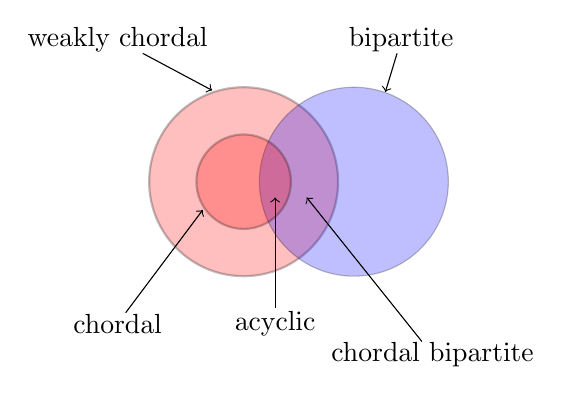
\begin{tikzpicture}[thick,scale=0.4]


\draw[ fill = red, opacity = 0.25] (0,0) circle (3);
\draw[ fill = blue, opacity = 0.25, thin] (3.5,0) circle (3);
\draw[ fill = red, opacity = 0.25] (0,0) circle (1.5);

\draw  (-4,4.5) node[words]{weakly chordal}
	edge [->, thin] (-1,2.9);

\draw  (-4,-4.5) node[words]{chordal}
	edge [->, thin] (-1.3,-0.9);

\draw (1,-4.5) node[words]{acyclic};
\draw node[words] (1,-4) {}
	edge [->, thin] (1,-.5);


\draw (6, -5.5) node[words]{chordal bipartite}
	edge[->, thin] (2,-.5);
\draw (5, 4.5) node[words]{bipartite}
	edge[->,thin] (4.5,2.85);

\end{tikzpicture}
 \end{center}
}

\bframe{Bisimplicial edges in chordal bipartite graphs}{
A {\it bisimplicial edge} in a bipartite graph $G = (A, B; E)$ is an edge $uv$ with the property that all edges between $N(u)$ and $N(v)$ are present.\pause\vskip 0.5 cm
\begin{center}\hspace{3cm}
\begin{overprint}
	\onslide<2>\hspace{3cm}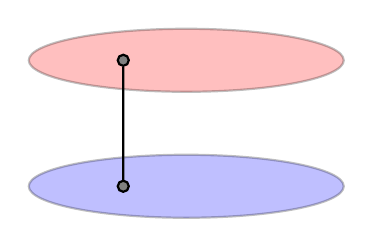
\begin{tikzpicture}[thick,scale=0.4]

\draw [fill = red, opacity = 0.25] (0,2) ellipse (5 and 1);
\draw [fill = blue, opacity = 0.25] (0,-2) ellipse (5 and 1);

\draw (-2,2) node[]{}
	edge[] (-2,-2);
\draw (-2,-2) node[]{};


\end{tikzpicture}\\
	\onslide<3>\hspace{3cm}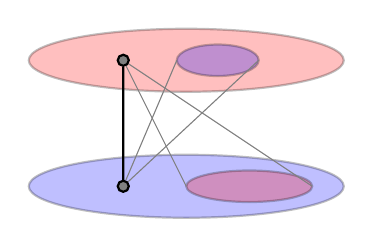
\begin{tikzpicture}[thick,scale=0.4]

\draw [fill = red, opacity = 0.25] (0,2) ellipse (5 and 1);
\draw [fill = blue, opacity = 0.25] (0,-2) ellipse (5 and 1);
\draw [fill = red, opacity = 0.25] (2,-2) ellipse (2 and 0.5);
\draw [fill = blue, opacity = 0.25] (1,2) ellipse (1.3 and 0.5);

\draw (-2,2) node[]{}
	edge[] (-2,-2)
	edge[thin, color = gray] (0, -2)
	edge[thin, color = gray] (4, -2);
\draw (-2,-2) node[]{}
	edge[thin, color = gray] (-.3, 2)
	edge[thin, color = gray] (2.3, 2);

%\draw (0.2,2)--(0.5,-2)--(1.8, 2)--(3.5, -2)--(0.2,2);

\end{tikzpicture}\\
	\onslide<4->\hspace{3cm}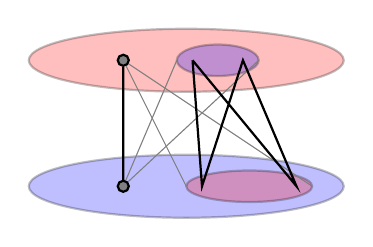
\begin{tikzpicture}[thick,scale=0.4]

\draw [fill = red, opacity = 0.25] (0,2) ellipse (5 and 1);
\draw [fill = blue, opacity = 0.25] (0,-2) ellipse (5 and 1);
\draw [fill = red, opacity = 0.25] (2,-2) ellipse (2 and 0.5);
\draw [fill = blue, opacity = 0.25] (1,2) ellipse (1.3 and 0.5);

\draw (-2,2) node[]{}
	edge[] (-2,-2)
	edge[thin, color = gray] (0, -2)
	edge[thin, color = gray] (4, -2);
\draw (-2,-2) node[]{}
	edge[thin, color = gray] (-.3, 2)
	edge[thin, color = gray] (2.3, 2);

\draw (0.2,2)--(0.5,-2)--(1.8, 2)--(3.5, -2)--(0.2,2);

\end{tikzpicture}
\end{overprint}
\end{center}\pause\pause\pause
Every induced subgraph of a chordal bipartite graph has a bisimplicial edge.  \pause If we remove a bisimplicial edge from a chordal bipartite graph, the resulting graph is chordal bipartite.\pause\vskip 0.5 cm
}
\bframe{An approach to MCM for chordal bipartite graphs}{
First, let us call an edge $e$ in $G$ {\it inert} if $\nu_c(G) = \nu_c(G-e)$. \pause\vskip 0.5 cm
Our strategy will be to remove inert bisimplicial edges until the maximum connected matching is easy to find. \pause\vskip 0.5 cm
\begin{prop}
Let $G = (A, B; E)$ be chordal bipartite.  A bisimplicial edge $e = uv$ is inert unless
	\begin{enumerate}
		\item $e$ is contained in every maximum connected matching.
		\item For any maximum connected matching $M$, every $f\neq e $ in $M$ has exactly one endpoint adjacent to $e$.
		\item  $N(e)$ is covered by $M$
	\end{enumerate}
\end{prop}


}

\bframe{Proof of 1: Inert, or in every max. conn. matching}{

\begin{overprint}
		\onslide<1>
			\begin{wrapfigure}{r}{4cm}\vspace{-20pt}\hspace{30pt}
			%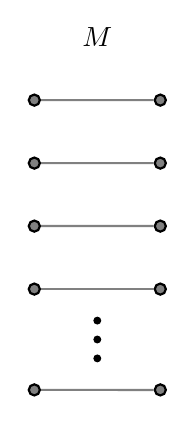
\begin{tikzpicture}[thick,scale=0.8]

\draw (0, 4) node[words]{$M$};


\draw (1, 3) node[]{}
	edge[color = gray] (-1, 3);
\draw (-1, 3) node[]{};
\draw (1, 2) node[]{}
	edge[color = gray] (-1, 2);
\draw (-1, 2) node[]{};
\draw (1, 1) node[]{}
	edge[color = gray] (-1, 1);
\draw (-1, 1) node[]{};
\draw (1, 0) node[]{}
	edge[color = gray] (-1, 0);
\draw (-1, 0) node[]{};


\draw (0,-0.5) node[dot]{};
\draw (0,-0.8) node[dot]{};
\draw (0,-1.1) node[dot]{};

\draw (1, -1.6) node[]{}
	edge[color = gray] (-1, -1.6);
\draw (-1, -1.6) node[]{};
\end{tikzpicture}
			\end{wrapfigure}
			  Let $e$ be non-inert, bisimplicial, and not contained in a maximum connected matching $M$.
		\onslide<2>
			\begin{wrapfigure}{r}{4cm}\vspace{-20pt}\hspace{30pt}
			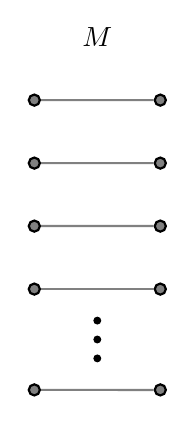
\begin{tikzpicture}[thick,scale=0.8]

\draw (0, 4) node[words]{$M$};


\draw (1, 3) node[]{}
	edge[color = gray] (-1, 3);
\draw (-1, 3) node[]{};
\draw (1, 2) node[]{}
	edge[color = gray] (-1, 2);
\draw (-1, 2) node[]{};
\draw (1, 1) node[]{}
	edge[color = gray] (-1, 1);
\draw (-1, 1) node[]{};
\draw (1, 0) node[]{}
	edge[color = gray] (-1, 0);
\draw (-1, 0) node[]{};


\draw (0,-0.5) node[dot]{};
\draw (0,-0.8) node[dot]{};
\draw (0,-1.1) node[dot]{};

\draw (1, -1.6) node[]{}
	edge[color = gray] (-1, -1.6);
\draw (-1, -1.6) node[]{};
\end{tikzpicture}
			\end{wrapfigure}
			  Let $e$ be non-inert, bisimplicial, and not contained in a maximum connected matching $M$.
		\onslide<3>
			\begin{wrapfigure}{r}{4cm}\vspace{-20pt}\hspace{30pt}
			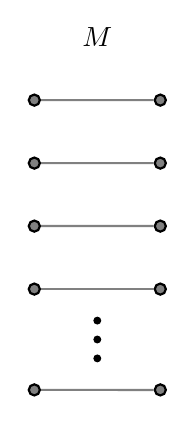
\begin{tikzpicture}[thick,scale=0.8]

\draw (0, 4) node[words]{$M$};


\draw (1, 3) node[]{}
	edge[color = gray] (-1, 3);
\draw (-1, 3) node[]{};
\draw (1, 2) node[]{}
	edge[color = gray] (-1, 2);
\draw (-1, 2) node[]{};
\draw (1, 1) node[]{}
	edge[color = gray] (-1, 1);
\draw (-1, 1) node[]{};
\draw (1, 0) node[]{}
	edge[color = gray] (-1, 0);
\draw (-1, 0) node[]{};


\draw (0,-0.5) node[dot]{};
\draw (0,-0.8) node[dot]{};
\draw (0,-1.1) node[dot]{};

\draw (1, -1.6) node[]{}
	edge[color = gray] (-1, -1.6);
\draw (-1, -1.6) node[]{};
\end{tikzpicture}
			\end{wrapfigure}
			If $e$ is not inert, then removing it must reduce the size of $M$. 
		\onslide<4>
			\begin{wrapfigure}{r}{4cm}\vspace{-20pt}\hspace{30pt}
			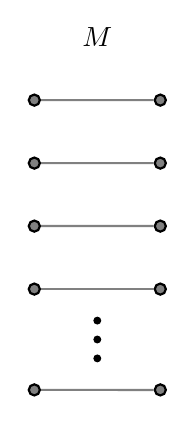
\begin{tikzpicture}[thick,scale=0.8]

\draw (0, 4) node[words]{$M$};


\draw (1, 3) node[]{}
	edge[color = gray] (-1, 3);
\draw (-1, 3) node[]{};
\draw (1, 2) node[]{}
	edge[color = gray] (-1, 2);
\draw (-1, 2) node[]{};
\draw (1, 1) node[]{}
	edge[color = gray] (-1, 1);
\draw (-1, 1) node[]{};
\draw (1, 0) node[]{}
	edge[color = gray] (-1, 0);
\draw (-1, 0) node[]{};


\draw (0,-0.5) node[dot]{};
\draw (0,-0.8) node[dot]{};
\draw (0,-1.1) node[dot]{};

\draw (1, -1.6) node[]{}
	edge[color = gray] (-1, -1.6);
\draw (-1, -1.6) node[]{};
\end{tikzpicture}
			\end{wrapfigure}
			If $e$ is not inert, then removing it must reduce the size of $M$. \vskip 0.5 cm
			So $e$ must ``connect'' two edges of $m$.
		\onslide<5>
			\begin{wrapfigure}{r}{4cm}\vspace{-20pt}\hspace{30pt}
			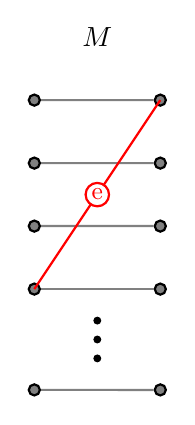
\begin{tikzpicture}[thick,scale=0.8]

\draw (0, 4) node[words]{$M$};


\draw (1, 3) node[]{}
	edge[color = gray] (-1, 3);
\draw (-1, 3) node[]{};
\draw (1, 2) node[]{}
	edge[color = gray] (-1, 2);
\draw (-1, 2) node[]{};
\draw (1, 1) node[]{}
	edge[color = gray] (-1, 1);
\draw (-1, 1) node[]{};
\draw (1, 0) node[]{}
	edge[color = gray] (-1, 0);
\draw (-1, 0) node[]{};

\draw[color = red] (1,3) -- (-1,0);
\draw[color = red] (0,1.5) node[lblvertex]{e};


\draw (0,-0.5) node[dot]{};
\draw (0,-0.8) node[dot]{};
\draw (0,-1.1) node[dot]{};

\draw (1, -1.6) node[]{}
	edge[color = gray] (-1, -1.6);
\draw (-1, -1.6) node[]{};
\end{tikzpicture}
			\end{wrapfigure}
			 If $e$ is not inert, then removing it must reduce the size of $M$. \vskip 0.5 cm
			So $e$ must ``connect'' two edges of $m$.
		\onslide<6>
			\begin{wrapfigure}{r}{4cm}\vspace{-20pt}\hspace{30pt}
			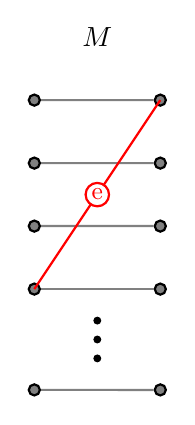
\begin{tikzpicture}[thick,scale=0.8]

\draw (0, 4) node[words]{$M$};


\draw (1, 3) node[]{}
	edge[color = gray] (-1, 3);
\draw (-1, 3) node[]{};
\draw (1, 2) node[]{}
	edge[color = gray] (-1, 2);
\draw (-1, 2) node[]{};
\draw (1, 1) node[]{}
	edge[color = gray] (-1, 1);
\draw (-1, 1) node[]{};
\draw (1, 0) node[]{}
	edge[color = gray] (-1, 0);
\draw (-1, 0) node[]{};

\draw[color = red] (1,3) -- (-1,0);
\draw[color = red] (0,1.5) node[lblvertex]{e};


\draw (0,-0.5) node[dot]{};
\draw (0,-0.8) node[dot]{};
\draw (0,-1.1) node[dot]{};

\draw (1, -1.6) node[]{}
	edge[color = gray] (-1, -1.6);
\draw (-1, -1.6) node[]{};
\end{tikzpicture}
			\end{wrapfigure}
			If $e$ is not inert, then removing it must reduce the size of $M$. \vskip 0.5 cm
			So $e$ must ``connect'' two edges of $m$. \vskip 0.5 cm
			But $e$ is bisimplicial, so the {\it other} edge in between the $M$ edges must be present.
		\onslide<7-8>
			\begin{wrapfigure}{r}{4cm}\vspace{-20pt}\hspace{30pt}
			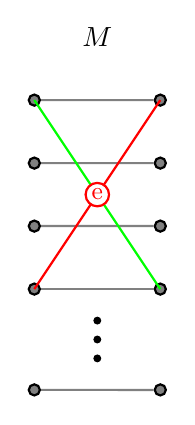
\begin{tikzpicture}[thick,scale=0.8]

\draw (0, 4) node[words]{$M$};


\draw (1, 3) node[]{}
	edge[color = gray] (-1, 3);
\draw (-1, 3) node[]{};
\draw (1, 2) node[]{}
	edge[color = gray] (-1, 2);
\draw (-1, 2) node[]{};
\draw (1, 1) node[]{}
	edge[color = gray] (-1, 1);
\draw (-1, 1) node[]{};
\draw (1, 0) node[]{}
	edge[color = gray] (-1, 0);
\draw (-1, 0) node[]{};

\draw[color = red] (1,3) -- (-1,0);
\draw[color = green] (-1,3)--(1,0);
\draw[color = red] (0,1.5) node[lblvertex]{e};


\draw (0,-0.5) node[dot]{};
\draw (0,-0.8) node[dot]{};
\draw (0,-1.1) node[dot]{};

\draw (1, -1.6) node[]{}
	edge[color = gray] (-1, -1.6);
\draw (-1, -1.6) node[]{};
\end{tikzpicture}
			\end{wrapfigure}
			If $e$ is not inert, then removing it must reduce the size of $M$. \vskip 0.5 cm
			So $e$ must ``connect'' two edges of $m$. \vskip 0.5 cm
			But $e$ is bisimplicial, so the {\it other} edge in between the $M$ edges must be present.
		\onslide<9->
			\begin{wrapfigure}{r}{4cm}\vspace{-20pt}\hspace{30pt}
			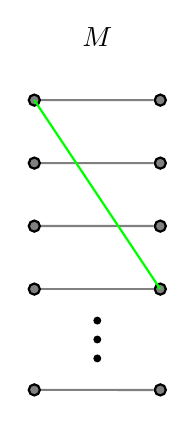
\begin{tikzpicture}[thick,scale=0.8]

\draw (0, 4) node[words]{$M$};


\draw (1, 3) node[]{}
	edge[color = gray] (-1, 3);
\draw (-1, 3) node[]{};
\draw (1, 2) node[]{}
	edge[color = gray] (-1, 2);
\draw (-1, 2) node[]{};
\draw (1, 1) node[]{}
	edge[color = gray] (-1, 1);
\draw (-1, 1) node[]{};
\draw (1, 0) node[]{}
	edge[color = gray] (-1, 0);
\draw (-1, 0) node[]{};

%\draw[color = red] (1,3) -- (-1,0);
\draw[color = green] (-1,3)--(1,0);
%\draw[color = red] (0,1.5) node[lblvertex]{e};


\draw (0,-0.5) node[dot]{};
\draw (0,-0.8) node[dot]{};
\draw (0,-1.1) node[dot]{};

\draw (1, -1.6) node[]{}
	edge[color = gray] (-1, -1.6);
\draw (-1, -1.6) node[]{};
\end{tikzpicture}
			\end{wrapfigure}
			If $e$ is not inert, then removing it must reduce the size of $M$. \vskip 0.5 cm
			So $e$ must ``connect'' two edges of $m$. \vskip 0.5 cm
			But $e$ is bisimplicial, so the {\it other} edge in between the $M$ edges must be present.
\end{overprint}
\pause\pause\pause\pause\pause\pause\pause \vskip 0.5 cm So $e$ is inert after all.
}

\bframe{Proof of 2: $e$ and $f$ in $M$ have one pair of adjacent ends}{

\begin{overprint}
		\onslide<1>
			\begin{wrapfigure}{r}{4cm}\vspace{-20pt}\hspace{30pt}
			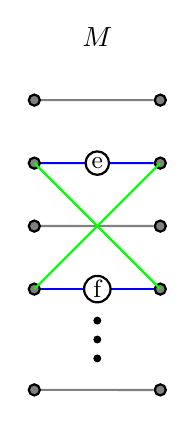
\begin{tikzpicture}[thick,scale=0.8]

\draw (0, 4) node[words]{$M$};


\draw (1, 3) node[]{}
	edge[color = gray] (-1, 3);
\draw (-1, 3) node[]{};
\draw (1, 2) node[]{}
	edge[color = blue] (-1, 2);
\draw (-1, 2) node[]{};
\draw (0,2) node[lblvertex]{e};
\draw (1, 1) node[]{}
	edge[color = gray] (-1, 1);
\draw (-1, 1) node[]{};
\draw (1, 0) node[]{}
	edge[color = blue] (-1, 0);
\draw (0,0) node[lblvertex]{f};
\draw (-1, 0) node[]{};

\draw[color = green] (1,2)--(-1,0);
\draw[color = green] (-1,2)--(1,0);


\draw (0,-0.5) node[dot]{};
\draw (0,-0.8) node[dot]{};
\draw (0,-1.1) node[dot]{};

\draw (1, -1.6) node[]{}
	edge[color = gray] (-1, -1.6);
\draw (-1, -1.6) node[]{};
\end{tikzpicture}
			\end{wrapfigure}
			 Suppose now that $e$ (bisimplicial) and $f$ are in some maximum connected matching $M$, and both edges between the endpoints of $e$ and $f$ are present.
		\onslide<2>
			\begin{wrapfigure}{r}{4cm}\vspace{-20pt}\hspace{30pt}
			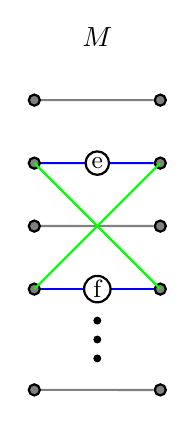
\begin{tikzpicture}[thick,scale=0.8]

\draw (0, 4) node[words]{$M$};


\draw (1, 3) node[]{}
	edge[color = gray] (-1, 3);
\draw (-1, 3) node[]{};
\draw (1, 2) node[]{}
	edge[color = blue] (-1, 2);
\draw (-1, 2) node[]{};
\draw (0,2) node[lblvertex]{e};
\draw (1, 1) node[]{}
	edge[color = gray] (-1, 1);
\draw (-1, 1) node[]{};
\draw (1, 0) node[]{}
	edge[color = blue] (-1, 0);
\draw (0,0) node[lblvertex]{f};
\draw (-1, 0) node[]{};

\draw[color = green] (1,2)--(-1,0);
\draw[color = green] (-1,2)--(1,0);


\draw (0,-0.5) node[dot]{};
\draw (0,-0.8) node[dot]{};
\draw (0,-1.1) node[dot]{};

\draw (1, -1.6) node[]{}
	edge[color = gray] (-1, -1.6);
\draw (-1, -1.6) node[]{};
\end{tikzpicture}
			\end{wrapfigure}
			Suppose now that $e$ (bisimplicial) and $f$ are in some maximum connected matching $M$, and both edges between the endpoints of $e$ and $f$ are present. \vskip 0.5 cm
We can replace $e$ and $f$ with these intermediary edges owing to the bisimpliciality of $e$.  
		\onslide<3>
			\begin{wrapfigure}{r}{4cm}\vspace{-20pt}\hspace{30pt}
			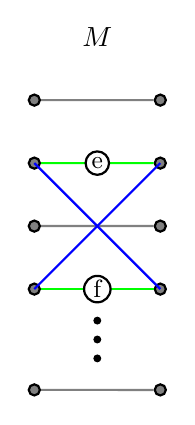
\begin{tikzpicture}[thick,scale=0.8]

\draw (0, 4) node[words]{$M$};


\draw (1, 3) node[]{}
	edge[color = gray] (-1, 3);
\draw (-1, 3) node[]{};
\draw (1, 2) node[]{}
	edge[color = green] (-1, 2);
\draw (-1, 2) node[]{};
\draw (0,2) node[lblvertex]{e};
\draw (1, 1) node[]{}
	edge[color = gray] (-1, 1);
\draw (-1, 1) node[]{};
\draw (1, 0) node[]{}
	edge[color = green] (-1, 0);
\draw (0,0) node[lblvertex]{f};
\draw (-1, 0) node[]{};

\draw[color = blue] (1,2)--(-1,0);
\draw[color = blue] (-1,2)--(1,0);


\draw (0,-0.5) node[dot]{};
\draw (0,-0.8) node[dot]{};
\draw (0,-1.1) node[dot]{};

\draw (1, -1.6) node[]{}
	edge[color = gray] (-1, -1.6);
\draw (-1, -1.6) node[]{};
\end{tikzpicture}
			\end{wrapfigure}
			Suppose now that $e$ (bisimplicial) and $f$ are in some maximum connected matching $M$, and both edges between the endpoints of $e$ and $f$ are present. \vskip 0.5 cm
We can replace $e$ and $f$ with these intermediary edges owing to the bisimpliciality of $e$.
		\onslide<4>
			\begin{wrapfigure}{r}{4cm}\vspace{-20pt}\hspace{30pt}
			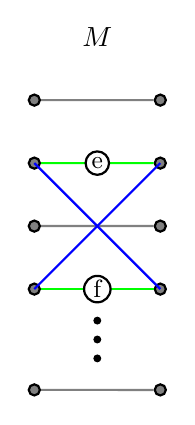
\begin{tikzpicture}[thick,scale=0.8]

\draw (0, 4) node[words]{$M$};


\draw (1, 3) node[]{}
	edge[color = gray] (-1, 3);
\draw (-1, 3) node[]{};
\draw (1, 2) node[]{}
	edge[color = green] (-1, 2);
\draw (-1, 2) node[]{};
\draw (0,2) node[lblvertex]{e};
\draw (1, 1) node[]{}
	edge[color = gray] (-1, 1);
\draw (-1, 1) node[]{};
\draw (1, 0) node[]{}
	edge[color = green] (-1, 0);
\draw (0,0) node[lblvertex]{f};
\draw (-1, 0) node[]{};

\draw[color = blue] (1,2)--(-1,0);
\draw[color = blue] (-1,2)--(1,0);


\draw (0,-0.5) node[dot]{};
\draw (0,-0.8) node[dot]{};
\draw (0,-1.1) node[dot]{};

\draw (1, -1.6) node[]{}
	edge[color = gray] (-1, -1.6);
\draw (-1, -1.6) node[]{};
\end{tikzpicture}
			\end{wrapfigure}
			Suppose now that $e$ (bisimplicial) and $f$ are in some maximum connected matching $M$, and both edges between the endpoints of $e$ and $f$ are present. \vskip 0.5 cm
We can replace $e$ and $f$ with these intermediary edges owing to the bisimpliciality of $e$. 	\vskip 0.5 cm So $e$ is inert.
\end{overprint}
}

\bframe{Proof  of 3: Every incident edge of $e$ is covered by $M$}{
\begin{overprint}
		\onslide<1>
			\begin{wrapfigure}{r}{4cm}\vspace{-20pt}\hspace{30pt}
			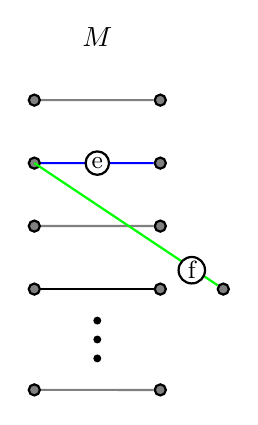
\begin{tikzpicture}[thick,scale=0.8]

\draw (0, 4) node[words]{$M$};


\draw (1, 3) node[]{}
	edge[color = gray] (-1, 3);
\draw (-1, 3) node[]{};
\draw (1, 2) node[]{}
	edge[color = blue] (-1, 2);
\draw (-1, 2) node[]{};
\draw (0,2) node[lblvertex]{e};
\draw (1, 1) node[]{}
	edge[color = gray] (-1, 1);
\draw (-1, 1) node[]{};
\draw (1, 0) node[]{}
	edge[] (-1, 0);]
\draw (-1,0) node[]{};

\draw (2,0) node[]{}
	edge[color = green] (-1,2);
\draw (1.5,0.3) node[lblvertex]{f};


\draw (0,-0.5) node[dot]{};
\draw (0,-0.8) node[dot]{};
\draw (0,-1.1) node[dot]{};

\draw (1, -1.6) node[]{}
	edge[color = gray] (-1, -1.6);
\draw (-1, -1.6) node[]{};
\end{tikzpicture}
			\end{wrapfigure}
			 Say that $e$ is bisimplicial, contained in maximum connected matching $M$, and has an incident edge $f$ not covered by $M$.
		\onslide<2>
			\begin{wrapfigure}{r}{4cm}\vspace{-20pt}\hspace{30pt}
			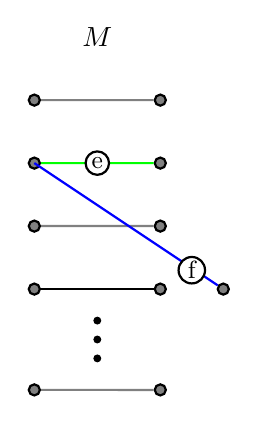
\begin{tikzpicture}[thick,scale=0.8]

\draw (0, 4) node[words]{$M$};


\draw (1, 3) node[]{}
	edge[color = gray] (-1, 3);
\draw (-1, 3) node[]{};
\draw (1, 2) node[]{}
	edge[color = green] (-1, 2);
\draw (-1, 2) node[]{};
\draw (0,2) node[lblvertex]{e};
\draw (1, 1) node[]{}
	edge[color = gray] (-1, 1);
\draw (-1, 1) node[]{};
\draw (1, 0) node[]{}
	edge[] (-1, 0);
\draw (-1,0) node[]{};

\draw (2,0) node[]{}
	edge[color = blue] (-1,2);
\draw (1.5,0.3) node[lblvertex]{f};


\draw (0,-0.5) node[dot]{};
\draw (0,-0.8) node[dot]{};
\draw (0,-1.1) node[dot]{};

\draw (1, -1.6) node[]{}
	edge[color = gray] (-1, -1.6);
\draw (-1, -1.6) node[]{};
\end{tikzpicture}
			\end{wrapfigure}
			 Say that $e$ is bisimplicial, contained in maximum connected matching $M$, and has an incident edge $f$ not covered by $M$. \vskip 0.5 cm
			We can switch out $e$ and switch in $f$, and $M$ remains connected. 
		\onslide<3>
			\begin{wrapfigure}{r}{4cm}\vspace{-20pt}\hspace{30pt}
			\begin{tikzpicture}[thick,scale=0.8]

\draw (0, 4) node[words]{$M$};


\draw (1, 3) node[]{}
	edge[color = gray] (-1, 3);
\draw (-1, 3) node[]{};
\draw (1, 2) node[]{}
	edge[color = green] (-1, 2);
\draw (-1, 2) node[]{};
\draw (0,2) node[lblvertex]{e};
\draw (1, 1) node[]{}
	edge[color = gray] (-1, 1);
\draw (-1, 1) node[]{};
\draw (1, 0) node[]{}
	edge[] (-1, 0);
\draw (-1,0) node[]{};

\draw (2,0) node[]{}
	edge[color = blue] (-1,2);
\draw (1.5,0.3) node[lblvertex]{f};


\draw (0,-0.5) node[dot]{};
\draw (0,-0.8) node[dot]{};
\draw (0,-1.1) node[dot]{};

\draw (1, -1.6) node[]{}
	edge[color = gray] (-1, -1.6);
\draw (-1, -1.6) node[]{};
\end{tikzpicture}
			\end{wrapfigure}
			 Say that $e$ is bisimplicial, contained in maximum connected matching $M$, and has an incident edge $f$ not covered by $M$. \vskip 0.5 cm
			We can switch out $e$ and switch in $f$, and $M$ remains connected.\vskip 0.5 cm
			Once more, $e$ is inert.
\end{overprint}
}


\bframe{Picture of a non-inert, bisimplicial edge}{
\pause
\begin{center}
\begin{overprint}
	\onslide<2>\hspace{4.5cm}\begin{tikzpicture}[thick,scale=0.4]

\draw[fill = red, opacity = 0.25]  (-2,0) ellipse(1 and 5);

\draw[fill = blue, opacity = 0.25] (2,0) ellipse (1 and 5);

\draw (-2,0) node[]{}
	edge[] (2,0);
\draw (2,0) node[]{};

\end{tikzpicture}
	\onslide<3>\hspace{4.5cm}\begin{tikzpicture}[thick,scale=0.4]

\draw[fill = red, opacity = 0.25]  (-2,0) ellipse(1 and 5);
\draw [fill = blue, opacity = 0.25](-2,-2.5) ellipse (0.5 and 1.5);
\draw[fill = blue, opacity = 0.25] (2,0) ellipse (1 and 5);
\draw[fill = red, opacity = 0.25] (2,2.5) ellipse (0.5 and 1.5);
\draw (-2,0) node[]{}
	edge[] (2,0);
\draw (2,0) node[]{};

\draw[color = gray] (-2,0)--(2,4);
\draw[color = gray] (-2,0)--(2,1);
\draw[color = gray] (2,0)--(-2,-1);
\draw[color = gray] (2,0)--(-2,-4);
\end{tikzpicture}
	\onslide<4>\hspace{4.5cm}\begin{tikzpicture}[thick,scale=0.4]

\draw[fill = red, opacity = 0.25]  (-2,0) ellipse(1 and 5);
\draw [fill = blue, opacity = 0.25](-2,-2.5) ellipse (0.5 and 1.5);
\draw[fill = blue, opacity = 0.25] (2,0) ellipse (1 and 5);
\draw[fill = red, opacity = 0.25] (2,2.5) ellipse (0.5 and 1.5);
\draw (-2,0) node[]{}
	edge[] (2,0);
\draw (2,0) node[]{};

\draw[color = gray] (-2,0)--(2,4);
\draw[color = gray] (-2,0)--(2,1);
\draw[color = gray] (2,0)--(-2,-1);
\draw[color = gray] (2,0)--(-2,-4);

\draw (-2,3.5)--(2,3.5);
\draw (-2,2.5)--(2,2.5);
\draw (-2,1.5)--(2,1.5);
\draw (-2,-3.5)--(2,-3.5);
\draw (-2,-2.5)--(2,-2.5);
\draw (-2,-1.5)--(2,-1.5);
\end{tikzpicture}
\end{overprint}
\end{center}

}

\bframe{Separable graphs}{Golumbic and Goss \cite{gg} showed that if $G$ is chordal bipartite and {\it separable}, then we can find two separable bisimplicial edges.  \pause\vskip 0.5 cm

If we have such a pair, it is clear from part 1 of the previous proposition that at least one is inert. \pause\vskip 0.5 cm

If we can efficiently determine which edge is inert, we can sequentially remove them until $G$ is no longer separable. \pause \vskip 0.5 cm

At this point we can apply a known maximum matching algorithm to obtain the maximum connected matching.
 }

\bframe{Reduction to a smaller problem}{

Suppose we have a separable pair $e = uv, f = xy$ of bisimplicial edges.\pause\vskip 0.5 cm
If $d(e) = d(f)$, then by part 1 of the previous proposition, both are inert and we can remove either one. \pause WLOG, assume $d(e) > d(f)$.  \pause \vskip 0.5 cm

We can say that $e$ is inert unless it looks like the picture we saw.  \pause I.e., connected matchings saturating the neighborhoods of the endpoints. \pause \vskip 0.5 cm

If $e$ has these matchings, we have found a larger connected matching than any that contain $f$, and $f$ is therefore inert.
}

\bframe{Perfect connected matching (PCM)}{
Now we have a smaller problem. \pause
\begin{framed}
  		Perfect connected matching (PCM)
  		\vskip 0.25 cm Instance: Bipartite graph $G = (A, B;E)$.
  		\newline Question: Is there a connected matching in $G$ that covers all of the vertices of $A$?
 	\end{framed}\pause

If we can solve SCM in polynomial time for $G$ chordal bipartite, then we can solve MCM in polynomial time for $G$ chordal bipartite.
}

\bframe{A sufficient condition for PCM}{
 
Suppose $|A| =n$.  \pause If there is a sequence of distinct vertices $b_1, b_2, \ldots, b_n$ from $B$ and subsets $S_1, S_2, \ldots ,S_n$ of $A$ such that\pause
	\begin{enumerate} 
		\item $S_n = A$, \pause
		\item $S_i \subseteq S_j$ whenever $i < j$, \pause
		\item $S_k \subseteq N(b_k)$ for all $1 \leq k \leq n$, and\pause
		\item $|S_k| \geq k$ for all $1 \leq k \leq n$\pause
	\end{enumerate}
then there is a connected matching covering $A$.
}

\bframe{Ordered connected matchings}{
A connected matching that has this property is called an {\it ordered } connected matching. PICTURE\pause\vskip 0.5 cm
Existence of this subgraph is equivalent to the condition as stated on the previous slide.
}

\bframe{A neccessary condition for PCM (chordal bipartite case)}{
In the chordal bipartite case, this condition is also neccessary.
\begin{prop}
	If $G$ is a chordal bipartite graph, then any connected matching $M$ in $G$ is ordered.
\end{prop}\pause\vskip 0.5 cm  
	We will show that a connected matching in a chordal bipartite graph has a vertex on each side that dominates the other side, and the ordering will follow.
}
\bframe{Proof}
{
 	We will proceed by induction on the size $n$ of the connected matching. \pause Small cases of $n = 1,2,3$ are obvious.  \pause \vskip 0.5 cm
	Assume now that the result holds for connected matchings up to $n-1$ edges, and let $M$ be a connected matching of $n$ edges in a chordal bipartite graph $G$.\pause \vskip 0.5 cm 

We will look at the subgraph $H$  induced by vertices covered by $M$.  \pause As we have observed previously, we can remove from $H$ any bisimplicial edges not contained in $M$ without reducing the size of $M$ \pause(or without introducing any new dominating vertices).  \pause  Remove such edges until any remaining bisimplicial edges are contained in $M$.
}

\bframe{Proof, cont.}{

The resulting graph is still chordal bipartite, so there exists a bisimplicial edge $xy$ contained in $M$. \pause If $y$ does not dominate $A$, look at the connected matching induced from $M$ by the neighbors of $x$ excluding $y$.  \pause \vskip 0.5 cm
Some $y'$ dominates the other side, which must contain all non-neighbors of $y$. \pause \vskip 0.5 cm The bisimpliciality of $xy$ ensures that $y'$ also dominates the neighbors of $y$.  \pause \vskip 0.5 cm Thus either $y$ or such a $y'$ dominates $A'$.  \pause (The argument can be repeated for $B'$ using $x$ instead of $y$.)  

}

\section{Future work}

\bframe{Where to go from here?}{

We have the following goals for the immediate future of this research:
\begin{itemize}\pause
	\item Improve partial result 3 of the extremal conjecture \pause
	\item Finish construction of a polytime algorithm for MCM on chordal bipartite graphs \pause
	\item Consider the complexity of weighted problem on chordal bipartite graphs, weighted and unweighted problems on weakly chordal graphs in general \pause
	\item Construct an efficient approximation algorithm for the general bipartite case 
\end{itemize}
}
\bframe{Thank you}{Questions?}

%\begin{bibsection}[Annotated Bibliography]\vspace{-\parskip} % This is the start of the bibliography. 
%	\begin{biblist}[\normalsize] % Replace the \bib entries with ones relevant to your problem.
							% The bulk of each entry can be copied and pasted from MathSciNet
							% ( http://www.ams.org/mathscinet/ ). When viewing the review of an
							% item you want to site, open the "Select alternative format" pull-down
							% and select AMSrefs.
							% Most likely, the only part you will need to change is the first parameter
							% after \bib. This is the internal name you use to cite the reference
							% with \cite. By default it will be the Mathematical Reviews number
							% (for example MR1375315). To make my life easier when I merge these all
							% into the summary document, please choose a name that begins with your
							% initials, followed by the number of problems you have submitted
							% (including this one).
							% For example, since this problem was submitted by Leonhard Euler and
							% since this is the first problem he is presenting, all citation names
							% begin with "le1". If this was his third problem, they would begin with
							% "le3".
%Z. Füredi, A. Gyárfás, G. Simonyi,  Connected matchings and Hadwiger's conjecture,  Combin. Probab. Comput., Problem Section, 14 (2005), 435--438.
%M. Kriesell, On seymour's strengthening of Hadwidger's conjecture for graphs with certain forbidden subgraphs 

%Mukhopadhyay, A. "The Square Root of a Graph." J. Combin. Th. 2, 290-295, 1967. 
\begin{thebibliography}{10}

\bib{MR671905}{article}{
   author={Duchet, P.},
   author={Meyniel, H.},
   title={On Hadwiger's number and the stability number},
   conference={
      title={Graph theory},
      address={Cambridge},
      date={1981},
   },
   book={
      series={North-Holland Math. Stud.},
      volume={62},
      publisher={North-Holland},
      place={Amsterdam},
   },
   date={1982},
   pages={71--73},
   review={\MR{671905 (84h:05074)}},
}

\bib{MR882610}{article}{
   author={Maffray, F.},
   author={Meyniel, H.},
   title={On a relationship between Hadwiger and stability numbers},
   journal={Discrete Math.},
   volume={64},
   date={1987},
   number={1},
   pages={39--42},
   issn={0012-365X},
   review={\MR{882610 (88g:05076)}},
   doi={10.1016/0012-365X(87)90238-X},
}


\bib{MR1411244}{article}{
   author={Toft, Bjarne},
   title={A survey of Hadwiger's conjecture},
   note={Surveys in graph theory (San Francisco, CA, 1995)},
   journal={Congr. Numer.},
   volume={115},
   date={1996},
   pages={249--283},
   issn={0384-9864},
   review={\MR{1411244 (97i:05048)}},
}
\bib{MR1654153}{article}{
   author={Reed, Bruce},
   author={Seymour, Paul},
   title={Fractional colouring and Hadwiger's conjecture},
   journal={J. Combin. Theory Ser. B},
   volume={74},
   date={1998},
   number={2},
   pages={147--152},
   issn={0095-8956},
   review={\MR{1654153 (99k:05079)}},
   doi={10.1006/jctb.1998.1835},
}
\bib{MR1844036}{article}{
   author={Kotlov, Andre{\u\i}},
   title={Matchings and Hadwiger's conjecture},
   note={Algebraic and topological methods in graph theory (Lake Bled,
   1999)},
   journal={Discrete Math.},
   volume={244},
   date={2002},
   number={1-3},
   pages={241--252},
   issn={0012-365X},
   review={\MR{1844036 (2002k:05087)}},
   doi={10.1016/S0012-365X(01)00087-5},
}



\bib{MR2163948}{article}{
   author={Cameron, Kathie},
   title={Connected matchings},
   conference={
      title={Combinatorial optimization---Eureka, you shrink!},
   },
   book={
      series={Lecture Notes in Comput. Sci.},
      volume={2570},
      publisher={Springer},
      place={Berlin},
   },
   date={2003},
   pages={34--38},
   review={\MR{2163948 (2006c:90072)}},
   %doi={10.1007/3-540-36478-1_5},
}

\bib{MR1979786}{article}{
   author={Klazar, Martin},
   title={Non-$P$-recursiveness of numbers of matchings or linear chord
   diagrams with many crossings},
   note={Formal power series and algebraic combinatorics (Scottsdale, AZ,
   2001)},
   journal={Adv. in Appl. Math.},
   volume={30},
   date={2003},
   number={1-2},
   pages={126--136},
   issn={0196-8858},
   review={\MR{1979786 (2004h:05006)}},
   doi={10.1016/S0196-8858(02)00528-6},
}



\bib{MR2070161}{article}{
   author={Plummer, Michael D.},
   author={Stiebitz, Michael},
   author={Toft, Bjarne},
   title={On a special case of Hadwiger's conjecture},
   journal={Discuss. Math. Graph Theory},
   volume={23},
   date={2003},
   number={2},
   pages={333--363},
   issn={1234-3099},
   review={\MR{2070161 (2005e:05055)}},
}

\bib{FGS}{article}{
   author={F\"{u}redi, Zolt\'{a}n},
   author={Gy{\'a}rf{\'a}s, Andr{\'a}s},
   author={Simonyi, G\'{a}bor}
   title={Connected matchings and Hadwiger's conjecture},
   journal={Combin. Probab. Comput.},
   part={Problem Section},
   volume={14},
   date={2005},
   pages={435--438},
}


\bib{MR2156345}{article}{
   author={Kawarabayashi, Ken-ichi},
   author={Plummer, Michael D.},
   author={Toft, Bjarne},
   title={Improvements of the theorem of Duchet and Meyniel on Hadwiger's
   conjecture},
   journal={J. Combin. Theory Ser. B},
   volume={95},
   date={2005},
   number={1},
   pages={152--167},
   issn={0095-8956},
   review={\MR{2156345 (2006b:05118)}},
   doi={10.1016/j.jctb.2005.04.001},
}


\bib{MR2249267}{article}{
   author={Gy{\'a}rf{\'a}s, Andr{\'a}s},
   author={Ruszink{\'o}, Mikl{\'o}s},
   author={S{\'a}rk{\"o}zy, G{\'a}bor N.},
   author={Szemer{\'e}di, Endre},
   title={One-sided coverings of colored complete bipartite graphs},
   conference={
      title={Topics in discrete mathematics},
   },
   book={
      series={Algorithms Combin.},
      volume={26},
      publisher={Springer},
      place={Berlin},
   },
   date={2006},
   pages={133--144},
   review={\MR{2249267 (2008c:05120)}},
   %doi={10.1007/3-540-33700-8_8},
}

\bib{FGS}{article}{
   author={Kriesell, Matthias},
   title={On Seymour's strengthening of Hadwiger's conjecture for graphs with certain forbidden subgraphs},
   journal={Discrete Mathematics},
   %volume={},
   date={2010},
   pages={435--438},
}

\bib{MR0297600}{article}{
   author={Chv{\'a}tal, V.},
   author={Erd{\H{o}}s, P.},
   title={A note on Hamiltonian circuits},
   journal={Discrete Math.},
   volume={2},
   date={1972},
   pages={111--113},
   issn={0012-365X},
   review={\MR{0297600 (45 \#6654)}},
}

\bib{MR1369063}{article}{
   author={Kim, Jeong Han},
   title={The Ramsey number $R(3,t)$ has order of magnitude $t\sp 2/\log t$},
   journal={Random Structures Algorithms},
   volume={7},
   date={1995},
   number={3},
   pages={173--207},
   issn={1042-9832},
   review={\MR{1369063 (96m:05140)}},
   doi={10.1002/rsa.3240070302},
}

\bib{MR0284366}{article}{
   author={Nash-Williams, C. St. J. A.},
   title={Edge-disjoint Hamiltonian circuits in graphs with vertices of
   large valency},
   conference={
      title={Studies in Pure Mathematics (Presented to Richard Rado)},
   },
   book={
      publisher={Academic Press},
      place={London},
   },
   date={1971},
   pages={157--183},
   review={\MR{0284366 (44 \#1594)}},
}

\bib{edhc}{article}{
	author={Christofides, Demetres},
	author={K\"{u}hn, Daniela},
	author={Osthus, Deryk},
	title={Edge-disjoint Hamilton cycles in graphs},
	date={31 Aug 2009},
	eprint={arXiv:0908.4572v1 [math.CO]},
	url={http://arxiv.org/abs/0908.4572},
}

\bib{MR1851303}{book}{
   author={Vazirani, Vijay V.},
   title={Approximation algorithms},
   publisher={Springer-Verlag},
   place={Berlin},
   date={2001},
   pages={xx+378},
   isbn={3-540-65367-8},
   review={\MR{1851303 (2002h:68001)}},
}

\bib{gg}{article}{
  author = {Golumbic, M.C.},
  author = {Goss, C.F.}
  title = {Perfect elimination and chordal bipartite graphs},
  year = {1978},
  volume = {2},
  journal = {J. Graph Theory},
  pages = {155-163}
}

\end{thebibliography}
\nocite{*}
\end{document}
